% SIAM Article Template
\documentclass[review,onefignum,onetabnum]{siamart190516}

% Information that is shared between the article and the supplement
% (title and author information, macros, packages, etc.) goes into
% ex_shared.tex. If there is no supplement, this file can be included
% directly.
% SIAM Shared Information Template
% This is information that is shared between the main document and any
% supplement. If no supplement is required, then this information can
% be included directly in the main document.


% Packages and macros go here
\usepackage{lipsum}
\usepackage{amsfonts}
\usepackage{graphicx}
\usepackage{epstopdf}
\usepackage{algorithmic}
\usepackage[T1]{fontenc}
\usepackage[utf8]{inputenc}
\ifpdf
  \DeclareGraphicsExtensions{.eps,.pdf,.png,.jpg}
\else
  \DeclareGraphicsExtensions{.eps}
\fi

% Add a serial/Oxford comma by default.
\newcommand{\creflastconjunction}{, and~}

% Used for creating new theorem and remark environments
\newsiamremark{remark}{Remark}
\newsiamremark{hypothesis}{Hypothesis}
\crefname{hypothesis}{Hypothesis}{Hypotheses}
\newsiamthm{claim}{Claim}

% Sets running headers as well as PDF title and authors
\headers{Adaptive methods using GP for regret-based estimates}{V. Trappler, E. Arnaud, A. Vidard}

% Title. If the supplement option is on, then "Supplementary Material"
% is automatically inserted before the title.
\title{Adaptive methods using GP for regret-based estimates\thanks{Document compiled on \today }% \thanks{Submitted to the editors DATE.
% \funding{This work was funded by the Fog Research Institute under contract no.~FRI-454.}}
}

% Authors: full names plus addresses.
\author{Victor Trappler\thanks{Univ. Grenoble-Alpes  (\email{victor.trappler@univ-grenoble-alpes.fr}, \url{http://vtrappler.github.io/}).}
\and Elise Arnaud \thanks{Univ Grenoble-Alpes} \and Arthur Vidard\footnotemark[3]}

\usepackage{amsopn}
\DeclareMathOperator{\diag}{diag}
\newcommand{\kk}{\theta}
\newcommand{\uu}{u}
\newcommand{\KK}{\theta}
\newcommand{\UU}{U}
\newcommand{\Kspace}{\Theta}
\newcommand{\Uspace}{\mathbb{U}}
\newcommand{\Xspace}{\mathbb{X}}
%%% Local Variables: 
%%% mode:latex
%%% TeX-master: "ex_article"
%%% End: 


% Optional PDF information
\ifpdf
\hypersetup{
  pdftitle={Adaptive methods using GP for regret-based estimates},
  pdfauthor={V. Trappler, E. Arnaud, and A. Vidard}
}
\fi

% The next statement enables references to information in the
% supplement. See the xr-hyperref package for details.

\externaldocument{ex_supplement}

% FundRef data to be entered by SIAM
%<funding-group specific-use="FundRef">
%<award-group>
%<funding-source>
%<named-content content-type="funder-name"> 
%</named-content> 
%<named-content content-type="funder-identifier"> 
%</named-content>
%</funding-source>
%<award-id> </award-id>
%</award-group>
%</funding-group>


\graphicspath{{/home/victor/collab_article/adaptive/figures/}}

\begin{document}

\maketitle

% REQUIRED
\begin{abstract}
  This is an example SIAM \LaTeX\ article. This can be used as a
  template for new articles.  Abstracts must be able to stand alone
  and so cannot contain citations to the paper's references,
  equations, etc.  An abstract must consist of a single paragraph and
  be concise. Because of online formatting, abstracts must appear as
  plain as possible. Any equations should be inline.
\end{abstract}

% REQUIRED
\begin{keywords}
  example, \LaTeX
\end{keywords}

% REQUIRED
\begin{AMS}
  68Q25, 68R10, 68U05
\end{AMS}

\section{Introduction}
\subsection{Contextual introduction}
\label{sec:context}


The introduction introduces the context and summarizes the
manuscript. It is importantly to clearly state the contributions of
this piece of work. The next two paragraphs are text filler,
generated by the \texttt{lipsum} package.

\lipsum[2-3]

% The outline is not required, but we show an example here.

\cite{trappler_robust_2020}
\subsection{Problem definition}
\label{sec:problem-definition}

In this work, we consider having an objective function $J$, that a
measure of error or discrepancy, thus lower values of $J$ are
preferable. The input can be split in two different components
\begin{itemize}
\item First, the control variable $\kk\in\Kspace$, whose value is up to the user 
\item Secondly, the environmental variable $\uu \in \Uspace$.
\end{itemize}

This function takes two arguments $\kk \in \Kspace$, and
$\uu \in \Uspace$:
\begin{equation}
  \label{eq:J_def}
  \begin{array}{rcl}
    \Kspace \times \Uspace  &  \longrightarrow & \mathbb{R} \\
    (\kk, \uu) & \longmapsto & J(\kk, \uu)
  \end{array}
\end{equation}




\section{Estimates based on the regret}
\label{sec:estim-based-regr}
\begin{definition}[Regret]
For a function $f: \Xspace \rightarrow \mathbb{R}$, we define the regret $r$ as
\begin{align}
  r_{\mathrm{A}}(x) &= f(x) - \min_{x\in\Xspace} f(x) = f(x) - f^* \\
  r_{\mathrm{R}}(x) &= \frac{f(x)}{\min_{x\in \Xspace}f(x)} = f(x)/f^*
\end{align}
where the subscript A refers to an \emph{additive} regret, while the
subscript R refers to the \emph{relative} regret.  
\end{definition}


As $J$ takes two inputs, we can then define the regret in this case:

\begin{definition}[Regret]
\begin{align}
  r_{\mathrm{A}}(\kk, \uu) &= J(\kk, \uu) - \min_{\kk\in\Kspace} J(\kk, \uu) = J(\kk, \uu) - J^*(\uu) \\
  r_{\mathrm{R}}(\kk, \uu) &= \frac{J(\kk, \uu)}{\min_{\kk\in \Kspace}J(\kk, \uu)} = J(\kk, \uu)/ J^*(\uu)
\end{align}
where $J^*: \uu \mapsto J^*(\uu)$ is the conditional minimiser, or
profile optimiser in~\cite{ginsbourger_bayesian_2014}.
\end{definition}

\section{GP formulation of regret-based problems}
\label{sec:GP_formul}
\subsection{Kriging equations}
\label{sec:krigin_eq}
Let us assume that the objective function $J$ has been evaluated on an
initial design $\mathcal{X}_0$ defined as
\begin{equation}
  \mathcal{X}_0 = \left\{\left(x_1,J(x_1)\right),\dots,\left(x_{n_0},J(x_{n_0})\right)\right\} \in \left(\left(\Kspace \times \Uspace\right) \times \mathbb{R} \right) ^{n_0}
\end{equation}
where $x_i = (\kk_i, \uu_i)$ for $1 \leq i \leq n_0$.

We define then
\begin{align}
  \mathbf{x} &= (x_1, \dots, x_{n_0})\in (\Kspace \times \Uspace)^{n_0} \\
  \mathbf{z} &= J(\mathbf{x}) = \left(J({x}_1),\dots, J(x_{n_0})\right) \in \mathbb{R}^{n_0}
\end{align}

\begin{equation}
  Z \mid \mathcal{X}_0 \sim \mathrm{GP}(m_{Z\mid\mathcal{X}_0}, C_{Z \mid \mathcal{X}_0})
\end{equation}

\begin{equation}
  \begin{pmatrix}
    Z(\mathbf{x}) \\
    Z(x)
  \end{pmatrix}
  \sim \mathcal{N}\left(
    \begin{pmatrix}
      \mu_Z \\ m_Z(x)
    \end{pmatrix} ;
    \begin{pmatrix}
      \mathbf{K}_{\mathcal{X}_{n_0}} & K_{\mathcal{X}_{n_0}}(x) \\
      K_{\mathcal{X}_{n_0}}(x)^T  & C_Z(x,x)
    \end{pmatrix}
    \right)
\end{equation}
\begin{align}
  Z(\mathbf{x}) &= \left(Z(x_1),\dots,Z(x_{n_0})\right) \\
  K_{\mathcal{X}_{n_0}}(x) &= \left(C_Z(x, x_1), \dots, C_Z(x, x_{n_0})\right) \\
  \mathbf{K}_{\mathcal{X}_{n_0}} &= \left(C(x_i, x_j) \right)_{1 \leq i,j \leq n_0}
\end{align}


The kriging prediction is defined as
\begin{align}
  m_{Z \mid \mathcal{X}_{n_0}}(x) = \mu_Z(x) + K_{\mathcal{X}_{n_0}}^T \mathbf{K}_{\mathcal{X}_{n_0}}^{-1} \left( \mathbf{z} - \mu_Z(x)\right)
\end{align}
when the experimental design is clear from the context, it will be
dropped from the notation.  Given a design and a GP, we can define a
measure of the prediction error associated with the conditioned GP by
integrating the prediction variance over. This is the IMSE
\begin{equation}
  \label{eq:IMSE_def}
  \mathrm{IMSE}(Z \mid \mathcal{X}) = \int_{\Xspace} \sigma^2_{Z \mid \mathcal{X}}(x)\,\mathrm{d}x
\end{equation}


\subsection{Regret}
In order to use the notion of regret, we have first to define the
Stochastic counterpart of $Z^*$: we consider the plug-in approximation
of the conditional minimum:
\begin{equation}
  m_Z^*(\uu) = \min_{\kk \in \Kspace} m_Z(\kk, \uu) = m_Z(\kk_Z^*(\uu),\uu)
\end{equation}
where $\kk^*_Z(\uu)$ is the conditional minimiser.

\begin{equation}
  \begin{pmatrix}
    Z(\kk, \uu) \\
    Z\left(\kk^*(\uu), \uu\right)
  \end{pmatrix}
  \sim
  \mathcal{N}\left(
    \begin{pmatrix}
      m_Z(\kk, \uu) \\
      m^*_Z(\uu)
    \end{pmatrix};
    \begin{pmatrix}
      \sigma^2_Z(\kk, \uu) & C\left((\kk, \uu),(\kk^*(\uu),\uu)\right) \\
      C\left((\kk, \uu),(\kk^*(\uu),\uu)\right)&  \sigma^2_{Z^*}(\uu) \\
    \end{pmatrix}
  \right)
\end{equation}
Finally, by scaling the random vector $\begin{pmatrix}
  Z(\kk, \uu) \\
  Z\left(\kk^*(\uu), \uu\right)
\end{pmatrix}$ by $\begin{bmatrix} 1 & - \alpha \end{bmatrix}$ and
translating by $-\beta$, we can define the random process $\Delta$,
indexed over $\Kspace \times \Uspace$ as
\begin{align}
  \Delta(\kk, \uu) & = Z(\kk, \uu) - \alpha Z^*(\uu) - \beta
\end{align}
As a linear combination of GP, $\Delta$ is a GP as well, and thus one of its property, is that at each point $(\kk, \uu) \in \Kspace \times \Uspace$,
\begin{align}
\Delta(\kk, \uu) \sim  \mathcal{N}\left(m_\Delta(\kk, \uu);\sigma^2_\Delta(\kk, \uu) \right)
\end{align}
where the mean and variance function are
\begin{align}
  m_{\Delta}(\kk, \uu) &= m_Z(\kk, \uu) - \alpha m_Z^*(\uu) - \beta \\
  \sigma^2_{\Delta}(\kk, \uu) &= \sigma^2_Z(\kk, \uu)  + \alpha^2  \sigma^2_{Z^*}(\uu) - 2 \alpha C\left((\kk, \uu),(\kk^*(\uu),\uu)\right)
\end{align}
\section{Exploration of the input space}
In this section, we will define and compare some exploration
strategies Let $\mathcal{X}$ be a design, we say that this design is
augmented by the couple $(x, z)$, when we append the pair
point/evaluation $(x, z)$:
\begin{equation}
  \mathcal{X} \cup \left\{(x, z)\right\}
\end{equation}
The evaluation $z$, which is supposed to represent $f(x)$, is not yet
known, but we do have the knowledge that $z \sim Z(x)$.


\begin{align}
  \mathbb{E}_{Z(x)}\left[\kappa(\mathcal{X} \cup \{(x, Z(x))\} \right] = \int_{\mathbb{R}} \kappa(\mathcal{X} \cup \{(x, z)\} \phi\left(\frac{z - m_Z(x)}{\sigma_Z(x)}\right) \,\mathrm{d}z
\end{align}
Finally, the augmented IMSE can be written as

\begin{equation}
  \mathrm{aIMSE}(x) = \int_{\mathbb{R}} \left(\int_{\Xspace} \sigma^2_{Z\mid \mathcal{X} \cup \{(x, z)\}}(\xi) \, \mathrm{d}\xi \right) \phi\left(\frac{z - m_Z(x)}{\sigma_Z(x)}\right) \,\mathrm{d}z
\end{equation}
\begin{figure}[ht]
  \centering
  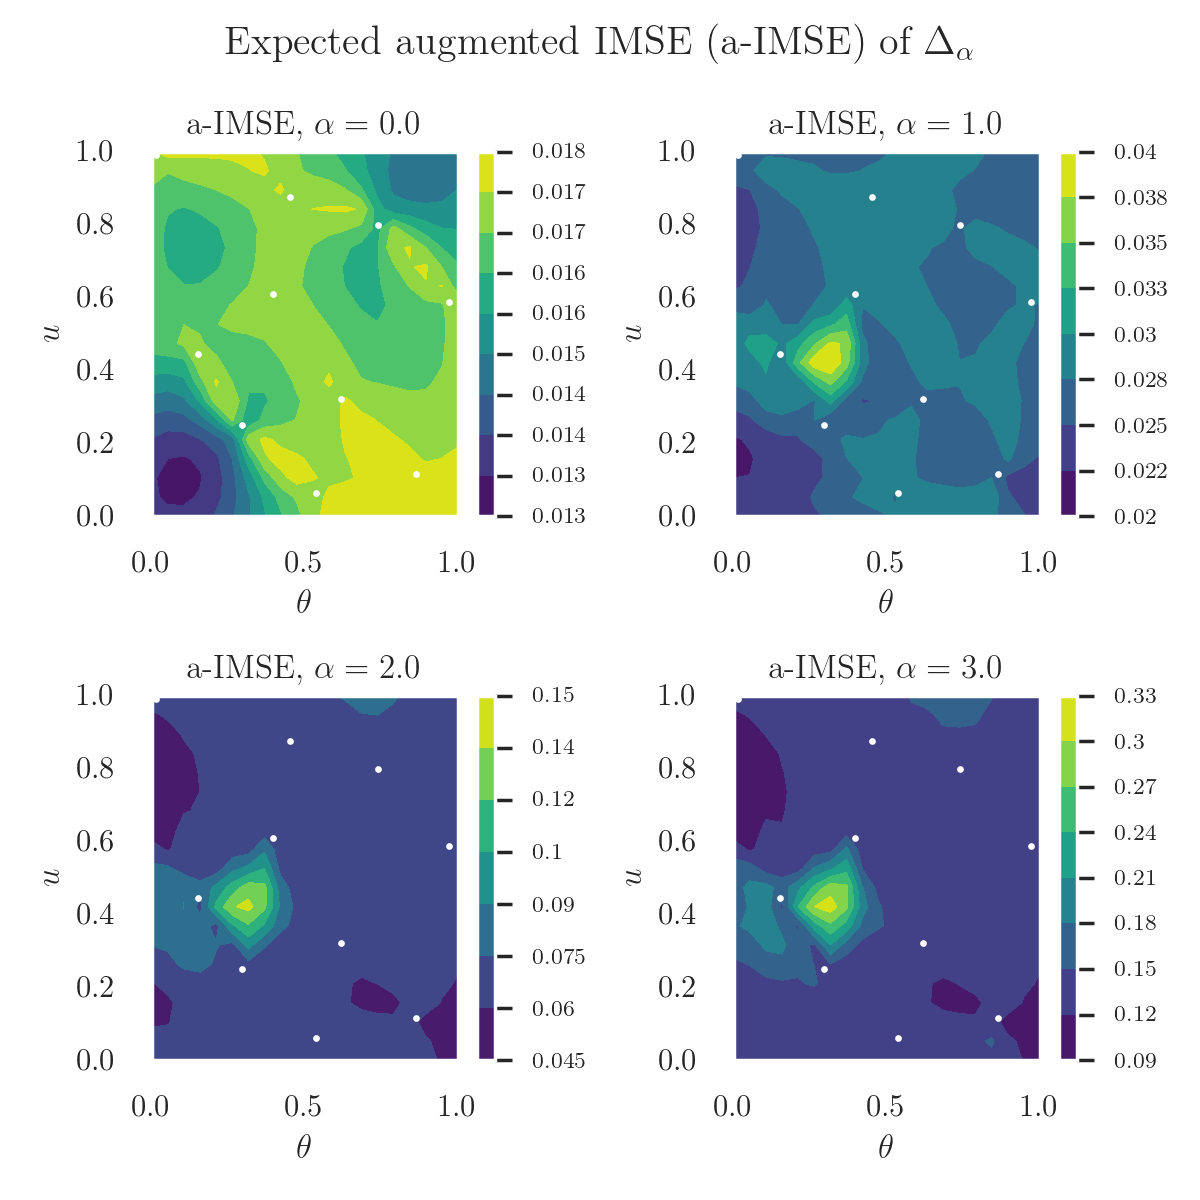
\includegraphics[width=\textwidth]{aIMSE_diff_alpha.png}
  \caption{\label{fig:aIMSE_diff_alpha} Expected augmented IMSE of
    $\Delta_{\alpha}$ for different $\alpha$. The case $\alpha=0$
    corresponds to the augmented IMSE of $Z$}
\end{figure}

\begin{itemize}
\item Maximize the prediction variance of $Z$
\item Maximize the prediction variance of $\Delta$
\item Minimize the augmented IMSE of $\Delta$
\end{itemize}

\begin{figure}[ht]
  \centering
  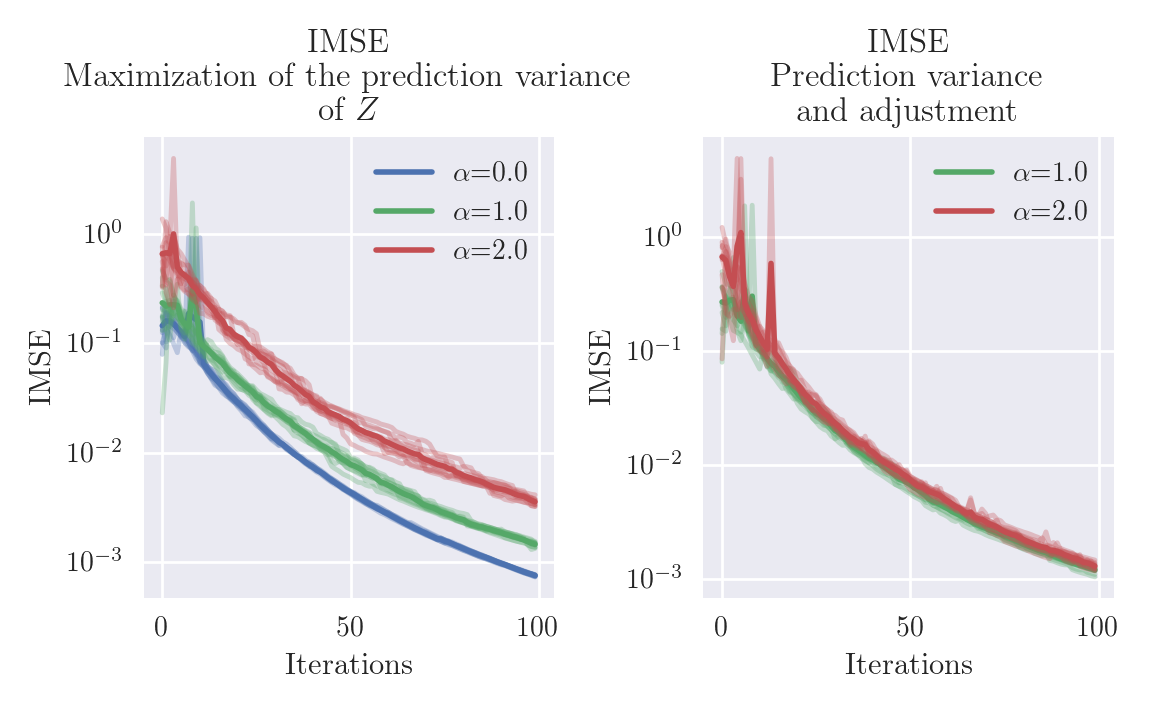
\includegraphics[width=\textwidth]{IMSE_predictionvariance_Delta_adjustment.png}
  \caption{\label{fig:IMSE_predictionvariance} }
\end{figure}


\section{Two-stage myopic method}


\section{Conclusions}
\label{sec:conclusions}

Some conclusions here.


\appendix
\section{An example appendix} 
azfgf



\section*{Acknowledgments}
We would like to acknowledge the assistance of volunteers in putting
together this example manuscript and supplement.

\bibliographystyle{siamplain}
\bibliography{/home/victor/acadwriting/bibzotero}
\end{document}
